\section{Diskusjon}
\label{section:diskusjon} 
\subsection{Numeriske metoder}
De numeriske metodene vi har brukt er Euler, RK4 og RKF45. Resultatene våre har vist at den enkleste og raskeste metoden er Euler. Euler har bare ett steg og er av første orden så denne vil være eksakt om funksjonene er en rett linje. RK4 og RKF45 består av flere steg og er av fjerde orden. Dette betyr at approksimasjonene vil være eksakt om den eksakte funksjonen er av grad 4 eller lavere. Ettersom resultatet for den eksakte løsningen i oppgave 2 inneholder funksjoner med sinus/cosinus svingninger er det ikke snakk om polynomer av orden 4 eller lavere. Cosinus og sinus funksjoner kan approksimeres som taylorrekker, men for at disse skal være nøyaktig må polynomet være av høy grad, noe som ikke kan approksimeres nøyaktig av RK4, RKF45 eller Euler. Dette kan vi se om vi sammenligner de numeriske løsningene mot den eksakte fra oppgave 2. Feilen er beregnet ved å sammenligne matrisene på samme måte som i RKF45-metoden: \newline
$E = \sqrt{trace(\Delta W^T \Delta W)}$ \newline 
Vi setter opp numerisk løsning på intervallet $0<t\leq50$ og steglengde 0.001. og plotter feilen på intervallet: \newline\newline
\begin{center}
\begin{minipage}{0.45\textwidth}
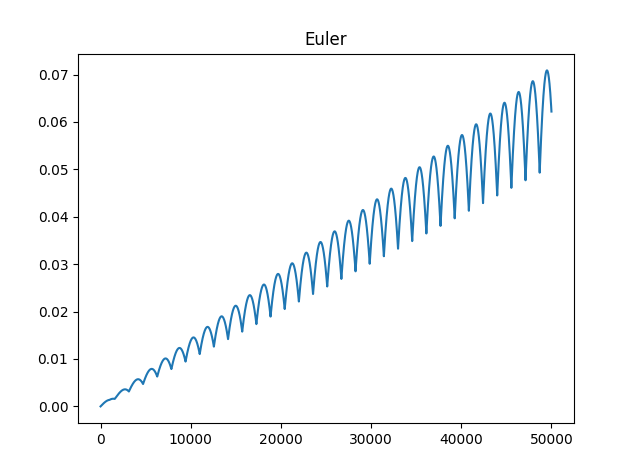
\includegraphics[width=\linewidth]{rapport/bilder/eulerError.png}
\end{minipage}\hfill
\begin{minipage}{0.45\textwidth}
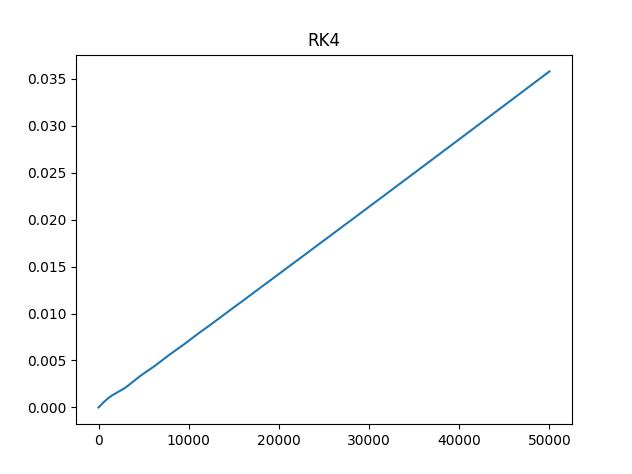
\includegraphics[width=\linewidth]{rapport/bilder/RK4Error.png} 
\end{minipage}
\begin{minipage}{0.45\textwidth}
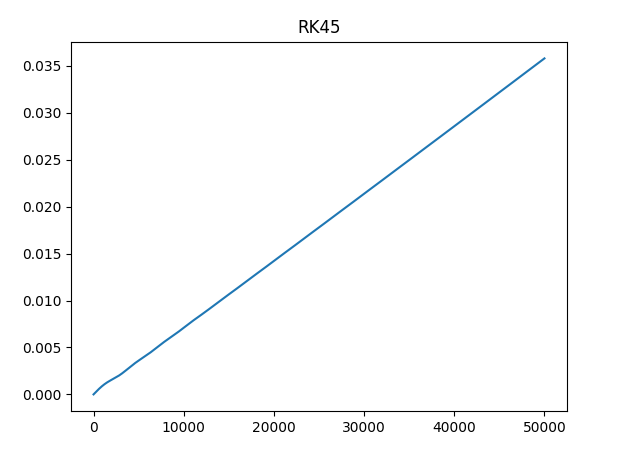
\includegraphics[width=\linewidth]{rapport/bilder/RK45.png} 
\end{minipage}
\captionof{figure}{Feilen for de ulike numeriske metodene}
\label{name_label}
\end{center}
Som vi kan se blir feilen større og større og er mer eller mindre helt lik for alle de numeriske løsningene. Dette tyder på at RK4 og RKF45 ikke er bedre eller mer nøyaktig enn Euler i dette tilfellet. Ettersom Euler er mye raskere og enklere vil dette være den beste metoden for denne situasjonen. Når det gjelder resultater fra oppgave 5 er det ikke godt å si hvilken metode som er best, ettersom vi ikke har en eksakt løsning for verdiene som er brukt i disse oppgavene. Det vi kan gjøre er å sammenligne animasjonene generert av de numeriske metodene.\newline \newline
I oppgave 6 sine resultater har vi lenker til videoer av simulasjonene. I oppgave a) kan vi se at RK4 og RKF45 roterer helt likt og går etterhvert over til å rotere om aksen med høyest treghetsmoment $(I_{zz})$, noe som i fysikken er et resultat av at den kinetiske energien avtar. Euler sin rotasjon holder seg derimot stabil. Ettersom den kinetiske energien i teorien ikke skal avta virker Euler sin rotasjon som den mest riktige løsningen, ettersom rotasjonens energi ikke avtar etterhvert. For videoene for oppgave b og c ser rotasjonene meget like ut for alle de numeriske løsningene, men vi vil se videre i kapittel \ref{section:rotasjon} at også her er det forskjell på energinivåene for RK4 og Euler.
\subsection{Rotasjon av T-nøkkelen}
\label{section:rotasjon}
Som vi ser fra videoene i kapittel \ref{section:oppgave6}, så roterer T-nøkkelen på ulike møter avhengig av hvilken akse den roterer om. Vi observerte i kapittel \ref{subseq:oppgavea} at rotasjonen for T-nøkkelen beregnet med RKF45 og RK4. Dette skjer pga. Mellomakse-teoremet som ble beskrevet i kapittel \ref{subseq:tennis}. Her beviste vi at t-nøkkelen vil rotere ustabilt om aksen med middels treghetsmoment ved å bruke Eulers likninger \cite{EULER:1} og at dreiemomentet $\tau=0$. Fra Oppgave 1c, så fant vi ut at treghetsmomentet $I$ blir
\begin{equation}
I = 
\begin{bmatrix}
982.27130302 & 0 & 0\\
0 & 722.67103008 & 0\\
0 & 0 & 1578.65030843\\
\end{bmatrix}.
\end{equation}
Siden rotasjonen er ustabil om $x$-aksen, og $I_{yy}<I_{xx}<I_{zz},$ så stemmer denne ustabile rotasjonen godt overens med mellomakse-teoremet. Vi kan også se av videoen for rotasjonen om $x$-aksen at t-nøkkelen begynner å rotere om $z$-aksen etter ca. $3$ minutter med spenning. Ettersom t-nøkkelen mister energi, så vil den begynne å rotere om aksen med høyest treghetsmoment. Dette er sant for ikke-stive legemer, men vi kan fortsatt observere dette fenomenet her.\cite{VERITASIUM:1} \newline\newline
Videre ser vi på rotasjonen om $y$-aksen. Her roterer t-nøkkelen på en relativt stabil måte, og for $z$-aksen er rotasjonen helt stabil. Denne stabiliteten reflekteres i den kinetiske energien for de ulike rotasjonene (se figur \ref{fig:energi})
\begin{figure}[!ht]
\begin{center}
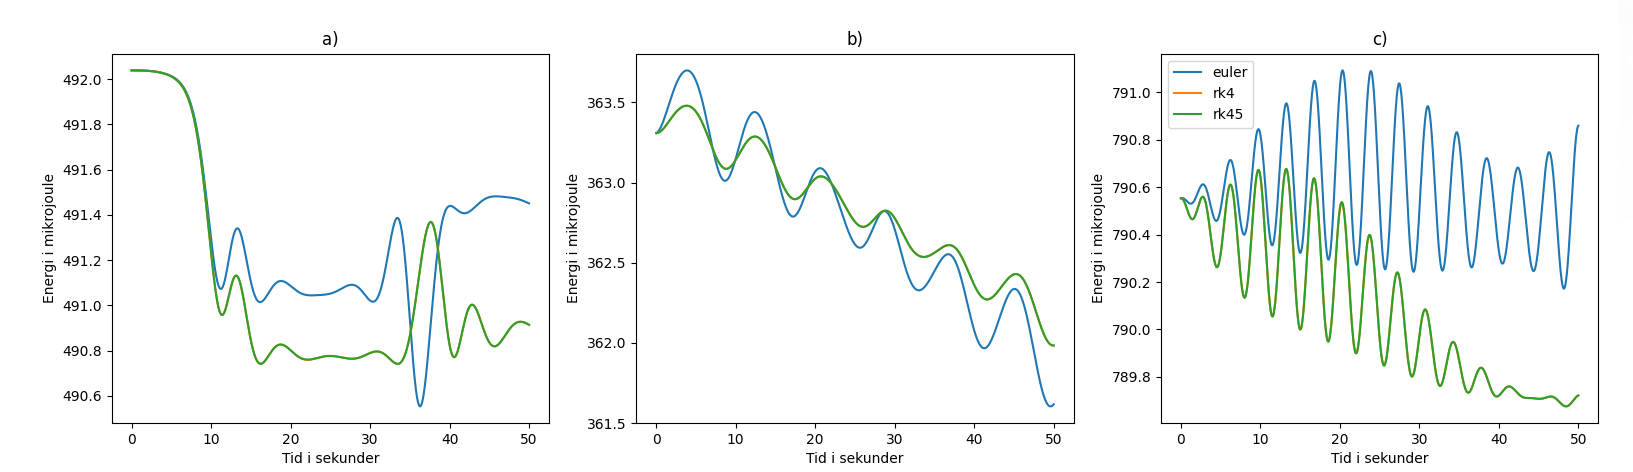
\includegraphics[width1.0\linewidth,height=0.4\linewidth]{rapport/bilder/energi.png}
\caption{Energien til t-nøkkelen beregnet med de 3 ulike numeriske metodene.}
\label{fig:energi}
\end{center}
\end{figure}
Her er energien i mikrojoule, og tiden er målt i sekunder. Som vi kan se, så endrer energien seg med ca. $1\text{ }\mu\text{J}.$ Den kinetiske energien endrer seg mest for rotasjonen om $x$-aksen, og minst for rotasjonen om $z$-aksen, noe som er å forvente ut i fra stabiliteten til rotasjonene ovenfor. Det er umulig å se den oransje grafen fordi det er fullstendig overlapp mellom energien til løsningen generert av RK4 og RKF45.
\subsection{Hva kunne vi undersøkt videre?}
I dette prosjektet har vi studert bevegelsene til en t-nøkkel gjennom de numeriske metodene Eulers-metode (kapittel \ref{section:oppgave3}), RK4 (kapittel \ref{section:oppgave4}) og RKF45 (kapittel \ref{section:oppgave5}). For å undersøke videre kunne vi forsøkt å bruke flere numeriske metoder og undersøkt nøyaktigheten på disse i forhold til de vi allerede har brukt.\newline\newline
Vi kunne for eksempel sett nærmere på Dormand-Prince-metoden \cite{DORMAND:1}. Dette er en variant av RKF45, der den også bruker variabel stegstørrelse. Dormand-Prince metoden har syv steg, men man bruker seks evalueringer. Dette er fordi den har egenskapen FSAL (First Same As Last), som betyr at den siste evaluering i hvert steg er den samme som den første i neste steg \cite{DORMAND:1}. Dormand-Prince metoden er laget for å minimere feilen for løsningen i 5. orden. Det er dette som skiller den fra RKF45, hvor man prøver å minimere feilen i 4. orden. \newline\newline
Noe annet vi kunne utforsket videre er hvilken effekt massen og størrelsen til t-nøkkelen har på bevegelsen. Vi kunne for eksempel endret på lengden til håndtaket til t-nøkkelen og sett på hvordan bevegelsen ville endret seg. Eller vi kunne sett hva som hadde skjedd hvis massen ikke var uniformt fordelt. Dermed kunne vi sett på effekten av å endre masse, lengde og radius til delene av t-nøkkelen og funnet ut hva som har størst påvirkning på resultatet.\newline
